\chapter{Постановка задачи декодирования}


%%%%%%%%%%%%%%%%%%%%%%%%%%%%%%%%%%%%%%%%%%%%%%%%
\section{Основные определения}
%%%%%%%%%%%%%%%%%%%%%%%%%%%%%%%%%%%%%%%%%%%%%%%%

%%%%%%%%%%%%%%%%%%%%%%%%%%%%%%%%%%%%%%%%%%%%%%%%
\section{Задача восстановления регрессии}
%%%%%%%%%%%%%%%%%%%%%%%%%%%%%%%%%%%%%%%%%%%%%%%%

Цель задачи регрессии~-- построить прогноз целевой переменной~$\by \in \bbR^r$ с $r$ компонентами по набору независимых переменных~$\bx \in \bbR^n$, где $n$~-- число признаков.
Предполагается, что между объектом~$\bx$ и целевой переменной~$\by$ существует линейная зависимость следующего вида:
\begin{equation}
\by = \bTheta \bx+ \boldsymbol{\varepsilon}.
\label{ch1:eq:model}
\end{equation}
Здесь $\bTheta \in \bbR^{r \times n}$~-- матрица параметров модели, $\boldsymbol{\varepsilon} \in \bbR^{r}$ представляет собой вектор остатков.
Дана наблюдаемая выборка $\left( \bX, \bY \right)$, где $\bX \in \bbR^{m \times n}$~-- матрица плана, $\bY \in \bbR^{m \times r}$~-- целевая матрица:
\begin{equation*}
\bX = [\bx_1, \dots, \bx_m]^{\T} =  [\bchi_1, \dots, \bchi_n]; \quad \bY = [\by_1, \dots, \by_m]^{\T} =  [\bnu_1, \dots, \bnu_r].
\end{equation*}
Столбцы~$\bchi_j, j=1, \dots, n$ матрицы~$\bX$ являются признаками объекта, столбцы~$\bnu_j, j=1, \dots, r$ матрицы ~$\bY$ являются целевыми столбцами.

Необходимо найти матрицу параметров модели~$\bTheta$ при известном наборе данных~$\left( \bX, \bY \right)$.
Оптимальные параметры~$\bTheta$ определяются минимизацией функции ошибки.
Определим квадратичную функцию потерь следующим образом:
\begin{equation}
\cL(\bTheta, \bX, \bY) = {\left\| \underset{m \times r}{\mathbf{Y}}  - \underset{m \times n}{\bX} \cdot \underset{r \times n}{\bTheta}^{\T} \right\| }_2^2 \rightarrow\min_{\bTheta}.
\label{ch1:eq:loss_function}
\end{equation}
Решением~\eqref{ch1:eq:loss_function} является следующая матрица:
\begin{equation*}
\bTheta = \bY^{\T} \bX (\bX^{\T} \bX)^{-1}.
\end{equation*}

Наличие линейной зависимости между столбцами матрицы~$\bX$ приводит к неустойчивому решению задачи оптимизации~\eqref{ch1:eq:loss_function}.
Если существует вектор~$\boldsymbol{\alpha} \neq \bZero_n$ такой, что $\bX \boldsymbol{\alpha}= \bZero_m$, то добавление~$\boldsymbol{\alpha}$ к любому столбцу матрицы~$\bTheta$ не меняет значение функции потерь~$\cL(\bTheta, \bX, \bY)$.
В этом случае матрица~$\bX^{\T} \bX$ близка к сингулярной и не обратима.
Чтобы избежать сильной линейной зависимости между признаками, используются методы снижения размерности и выбора признаков.

%%%%%%%%%%%%%%%%%%%%%%%%%%%%%%%%%%%%%%%%%%%%%%%%
\section{Метод проекции в скрытое пространство}
%%%%%%%%%%%%%%%%%%%%%%%%%%%%%%%%%%%%%%%%%%%%%%%%

Для устранения линейной зависимости и снижения размерности входного пространства объектов широко используется метод главных компонент~(PCA). 
Метод PCA находит низкоразмерное представление матрицы~$\bX = \bT \bP^{\T}$, такое что новое представление~$\bT \in \bbR^{m \times l}$ содержит максимальную долю дисперсии исходной матрицы.
Основным недостатком метода PCA является отсутствие учёта взаимосвязи между признаками~$\bchi_j$ и целевыми векторами~$\bnu_j$.
Алгоритм частичных наименьших квадратов проецирует матрицу плана~$\bX$ и целевую матрицу~$\bY$ в скрытое пространство малой размерностью~$l$ ($l < n$).
Алгоритм PLS находит в скрытом пространстве матрицы~$\bT, \bU \in \mathbb{R}^{m \times l}$, которые лучше всего описывают оригинальные матрицы~$\bX$ и~$\bY$. 
При этом PLS максимизирует взаимосвязь между $\bT$ и $\bU$.

Матрица плана~$\bX$ и целевая матрица~$\bY$ проецируются в скрытое пространство следующим образом:
\begin{align}
\label{ch1:eq:PLS_X}
\underset{m \times n}{\bX} 
&= \underset{m \times l}{\bT} \cdot \underset{l \times n}{\bP^{\T}} + \underset{m \times n}{\bF} 
= \sum_{k=1}^l \underset{m \times 1}{\bt_k} \cdot \underset{1 \times n}{\bp_k^{\T}} + \underset{m \times n}{\bF},\\
\label{ch1:eq:PLS_Y}
\underset{m \times r}{\bY} 
&= \underset{m \times l}{\bU} \cdot \underset{l \times r}{\bQ^{\T}} + \underset{m \times r}{\bE}
=  \sum_{k=1}^l  \underset{m \times 1}{\bu_k} \cdot \underset{1 \times r}{\bq_k^{\T}} +  \underset{m \times r}{\bE}.
\end{align}
Здесь $\bT$ и $\bU$~-- образы исходных матриц в скрытом пространстве, причём столбцы матрицы $\bT$ ортогональны; $\bP$ и $\bQ$~-- матрицы перехода; $\bE$ и $\bF$~-- матрицы остатков. 
Алгоритм PLS максимизирует линейную зависимость между столбцами матриц~$\bT$ и~$\bU$
\begin{equation*}
\bU \approx \bT \bB, \quad \bB = \text{diag}(\beta_k), \quad \beta_k = \bu_k^{\T}\bt_k / (\bt_k^{\T}\bt_k).
\end{equation*}

Псевдокод метода регрессии PLS приведен в алгоритме~\ref{PLSR_code}.
Алгоритм итеративно на каждом из $l$ шагов вычисляет по одному столбцу $\bt_k$, $\bu_k$, $\bp_k$, $\bq_k$ матриц $\bT$, $\bU$, $\bP$, $\bQ$ соответственно. 
После вычисления следующего набора векторов из матриц $\bX$, $\bY$ вычитаются очередные одноранговые аппроксимации. 
При этом предполагается, что исходные матрицы~$\bX$ и~$\bY$ нормированы (имеют нулевое среднее и единичное среднее отклонение).

\begin{algorithm}[h]
	\caption{Алгоритм PLS}
	\label{PLSR_code}
	\begin{algorithmic}[1]
		\REQUIRE $\bX, \bY, l$;
		\ENSURE $\bT, \bP, \bQ$;
		\STATE нормировать матрицы $\bX$ и $\bY$ по столбцам
		\STATE инициализировать $\bu_0$ (первый столбец матрицы $\bY$)
		\STATE $\bX_1 = \bX; \bY_1 = \bY$
		\FOR{$k=1,\dots, l$}
		\REPEAT
		\vspace{0.1cm}
		\STATE $\bw_k := \bX_k^{\T} \bu_{k-1} / (\bu_{k-1}^{\T} \bu_{k-1}); \quad \bw_k: = \frac{\bw_k}{\| \bw_k \|}$
		\vspace{0.1cm}
		\STATE $\bt_k := \bX_k \bw_k$
		\vspace{0.1cm}
		\STATE $\bc_k := \bY_k^{\T} \bt_k / (\bt_k^{\T} \bt_k); \quad \bc_k: = \frac{\bc_k}{\| \bc_k \|}$
		\vspace{0.1cm}
		\STATE $\bu_k := \bY_k \bc_k$
		\UNTIL{$\bt_k$ не стабилизируется}
		\vspace{0.1cm}
		\STATE $\bp_k:= \bX_k^{\T}\bt_k/(\bt_k^{\T}\bt_k),\ 
		\bq_k := \bY_k^{\T}\bt_k/(\bt_k^{\T}\bt_k)$
		\vspace{0.2cm}
		\STATE $\bX_{k+1} :=  \bX_k - \bt_k \bp_k^{\T}$
		\vspace{0.2cm}
		\STATE $\bY_{k + 1} :=  \bY_k - \bt_k \bq_k^{\T}$ 
		\ENDFOR
	\end{algorithmic}
\end{algorithm}

Вектора $\bt_k$ и $\bu_k$ из внутреннего цикла алгоритма~\ref{PLSR_code}
содержат информацию о матрице объектов $\bX$ и матрице ответов $\bY$ соответственно. 
Блоки из шагов (6)-(7) и шагов (8)-(9)~--- аналоги алгоритма PCA для матриц $\bX$ и $\bY$~\cite{geladi1988pls}. 
Последовательное выполнение блоков позволяет учесть взаимную связь между матрицами $\bX$ и $\bY$.

Теоретическое обоснование алгоритма PLS следует из следующих утверждений.
\begin{statement}
	Максимизации ковариации между векторами $\bt_k$ и $\bu_k$ сохраняет дисперсию матриц~$\bX$ и~$\bY$ и учитывает их линейную зависимость.
\end{statement}
\begin{proof}
Утверждение следует из равенства
\[
\text{cov} (\bt_k, \bu_k) = \text{corr} (\bt_k, \bu_k) \cdot \sqrt{\text{var}(\bt_k)} \cdot \sqrt{\text{var}(\bu_k)}.
\]
Максимизация дисперсий векторов $\bt_k$ и $\bu_k$ отвечает за сохранение информации об исходных матрицах, 
корреляция между векторами отвечает взаимосвязи между $\bX$ и~$\bY$. 
\end{proof}

Во внутреннем цикле алгоритма вычисляются нормированные вектора весов $\bw_k$ и $\bc_k$. 
Из данных векторов строятся матрицы весов $\bW$ и $\bC$ соответственно.

\begin{statement}
	В результате выполнения внутреннего цикла вектора $\bw_k$ и $\bc_k$ будут собственными векторами матриц $\bX_k^{\T} \bY_k \bY_k^{\T} \bX_k$ и $\bY_k^{\T} \bX_k \bX_k^{\T} \bY_k$, соответствующими максимальным собственным значениям.
	
	\begin{equation*}
	\bw_k \varpropto \bX_k^{\T} \bu_{k-1} \varpropto \bX_k^{\T} \bY_k \bc_{k-1} \varpropto \bX_k^{\T} \bY_k \bY_k^{\T} \bt_{k-1} \varpropto \bX_k^{\T} \bY_k \bY_k^{\T} \bX_k \bw_{k-1},
	\end{equation*}
	\begin{equation*}
	\bc_k \varpropto \bY_k^{\T} \bt_k \varpropto \bY_k^{\T} \bX_k \bw_k \varpropto \bY_k^{\T} \bX_k \bX_k^{\T} \bu_{k-1} \varpropto \bY_k^{\T} \bX_k \bX_k^{\T} \bY_k \bc_{k-1},
	\end{equation*}
	где символ $\varpropto$ означает равенство с точностью до мультипликативной константы. 
	\label{st:eig}
\end{statement}
\begin{proof}
Утверждение следует из того факта, что правила обновления векторов $\bw_k$, $\bc_k$ совпадают с итерацией алгоритма поиска максимального собственного значения. 
Данный алгоритм основан на следующем факте.

Если матрица $\mathbf{A}$ диагонализуема, $\bx$~--- некоторый вектор, то

\[
\lim_{k \rightarrow \infty} \mathbf{A}^k \bx = \lambda_{\max}(\mathbf{A}) \cdot \mathbf{v}_{\max},
\]
где $ \lambda_{\max} (\mathbf{A})$~--- максимальное собственное значение матрицы $\mathbf{A}$, $\mathbf{v}_{\max}$~---собственный вектор матрицы $\mathbf{A}$, соответствующий~$\lambda_{\max} (\mathbf{A})$.

\end{proof}

\begin{statement}
	Обновление векторов по шагам (6)--(9) алгоритма~\ref{PLSR_code} соответствует максимизации ковариации между векторами~$\bt_k$ и~$\bu_k$.
\end{statement}
\begin{proof}
Максимальная ковариация между векторами~$\bt_k$ и~$\bu_k$ равна максимальному собственному значению матрицы~$\bX_k^{\T} \bY_k \bY_k^{\T} \bX_k$:
\begin{align*}
\max_{\bt_k, \bu_k}  \text{cov} (\bt_k, \bu_k)^2 &= \max_{\substack{\|\bw_k\|=1 \\ \|\bc_k\| = 1}} \text{cov} \left( \bX_k \bw_k, \bY_k \bc_k \right)^2 = \max_{\substack{\|\bw_k\|=1 \\ \|\bc_k\| = 1}} \text{cov} \left(\bc_k^{\T}  \bY_k^{\T} \bX_k \bw_k \right)^2 = \\
&= \max_{\|\bw_k\| = 1} \text{cov} \left\|\bY_k^{\T} \bX_k \bw_k \right\|^2 = \max_{\|\bw_k\| = 1} \bw_k^{\T} \bX_k^{\T} \bY_k \bY_k^{\T} \bX_k \bw_k = \\
& = \lambda_{\max} \left( \bX_k^{\T} \bY_k \bY_k^{\T} \bX_k \right),
\end{align*}
где~$\lambda_{\max} (\mathbf{A})$~--- максимальное собственное значение матрицы $\mathbf{A}$.
Применяя утверждение~\ref{st:eig}, получаем требуемое.
\end{proof}

После завершения внутреннего цикла на шаге (11) вычисляются вектора $\bp_k$, $\bq_k$ проецированием столбцов матриц $\bX_k$ и $\bY_k$ на вектор $\bt_k$. 
Для перехода на следующий шаг необходимо вычесть из матриц $\bX_k$ и $\bY_k$ одноранговые аппроксимации $\bt_k \bp_k^{\T}$ и $\bt_k \bq_k^{\T}$
\begin{equation*}
\bX_{k + 1} = \bX_{k} - \bt_k \bp_k^{\T} = \bX - \sum_k \bt_k \bp_k^{\T},
\end{equation*}
\begin{equation*}
\bY_{k + 1} = \bY_{k} - \bt_k \bq_k^{\T} = \bY - \sum_k \bt_k \bq_k^{\T}.
\end{equation*}
При этом каждый следующий вектор~$\bt_k$ оказывается ортогонален всем векторам~$\bt_i$, $i=1, \dots, k$.

На Рис.~\ref{ch1:fig:PLSFigure} продемонстрирован результат работы алгоритма PLS для случая, когда размерности пространств объектов, ответов и латентного пространства равны 2 ($n = r = l = 2$).
Синими и зелёными точками изображены объекты~$\bx_i$ и целевые переменные~$\by_i$. 
Точки сгенерированы из нормального распределения с нулевым матожиданием. 
Красным контуром показаны линии уровня матриц ковариаций распределений. 
Черным изображены единичные окружности. 
Красные стрелки соответствуют главным компонентам матриц~$\bX$ и~$\bY$. 
Черные стрелки соответствуют векторам матриц~$\bW$ и~$\bC$ алгоритма PLS. 
Вектора $\bt_k$ и $\bu_k$~--- проекции матриц~$\bX_k$ и~$\bY_k$ на вектора~$\bw_k$ и~$\bc_k$ соответственно и изображены черными плюсами. 
Учёт взаимной связи между матрицами~$\bX$ и~$\bY$ отклоняет вектора~$\bw_k$ и~$\bc_k$ от направления главных компонент. 
Вектора~$\bw_k$ отклоняются незначительно. 
На первой итерации~$\bc_1$ близок к~$\textit{pc}_1$, но вектора~$\bc_k$, найденные на следующих итерациях могут оказаться сильно коррелированными. Это происходит в следствие того, что из матрицы~$\bY$ на каждом шаге вычитается одноранговая аппроксимация, найденная в пространстве матрицы~$\bX_k$.
\begin{figure}[h]
	\centering
	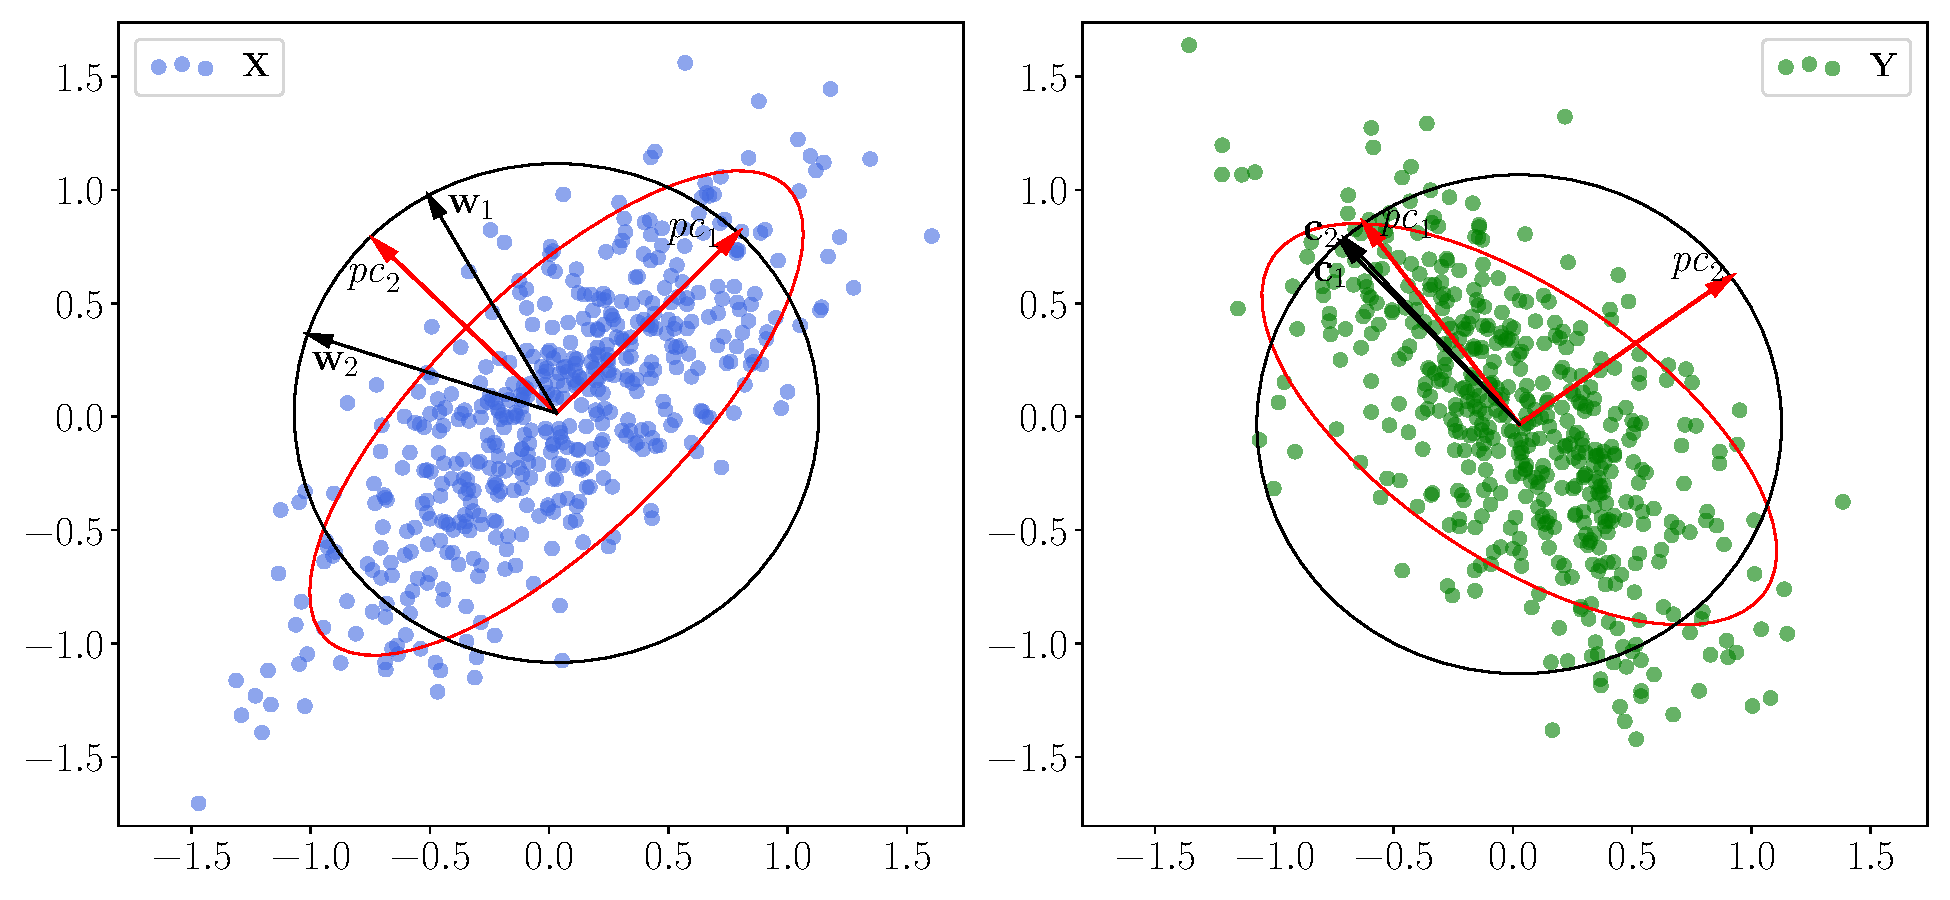
\includegraphics[width=\linewidth]{figs/ch1/PLSFigure}
	\caption{Иллюстрация алгоритма PLS}
	\label{ch1:fig:PLSFigure}
\end{figure}

Для получения прогнозов модели и нахождения параметров модели 
домножим справа формулу~\eqref{ch1:eq:PLS_X} на матрицу $\bW$. Строки матрицы невязок $\bE$ ортогональны столбцам матрицы $\bW$, поэтому 
\[
\bX \bW = \bT \bP^{\T} \bW.
\] 

Линейное преобразование между объектами в исходном и латентном пространстве имеет вид
\begin{equation}
\bT = \bX \bW^*,
\label{ch1:eq:W*}
\end{equation}
где $\bW^* = \bW (\bP^{\T} \bW)^{-1}$. 

Матрица параметров модели~\ref{ch1:eq:model} находится из уравнений~\eqref{ch1:eq:PLS_Y},~\eqref{ch1:eq:W*}
\begin{equation*}
\bY = \bT \bQ^{\T} + \bE = \bX \bW^* \bQ^{\T} + \bE = \bX \bTheta + \bE.
\label{ch1:eq:pls_model}
\end{equation*}
Таким образом, параметры модели~\eqref{ch1:eq:model} равны
\begin{equation}
\bTheta = \bW (\bP^{\T} \bW)^{-1} \bQ^{\T}.
\label{ch1:eq:model_parameters}
\end{equation}

Финальная модель~\eqref{ch1:eq:pls_model} является линейной, низкоразмерной в скрытом пространстве. 
Это снижает избыточность данных и повышает стабильность модели.

%%%%%%%%%%%%%%%%%%%%%%%%%%%%%%%%%%%%%%%%%%%%%%%%
\section{Вычислительный эксперимент}
%%%%%%%%%%%%%%%%%%%%%%%%%%%%%%%%%%%%%%%%%%%%%%%%

Временные ряды электроэнергии состоят из почасовых записей (52512 наблюдений). 
Строка матрицы~$\bX$~--– локальная история сигнала за одну неделю $n = 24 \times 7$. Строка матрицы~$\bY$~--- локальный прогноз потребления электроэнергии в следующие 24 часа $r = 24$. В этом случае матрицы~$\bX$ и~$\bY$ являются авторегрессионными матрицами.

Вычислительный эксперимент также проводился на данных электрокортикограмм (ECoG) из проекта NeuroTycho~\cite{shimoda2012decoding}.
Данные ECoG состоят из 32-канальных сигналов напряжения, снятых с головного мозга.
Цель состоит в предсказании по входному сигналу ECoG 3D позиции рук в последующие моменты времени.
Исходные сигналы напряжения преобразуются в пространственно-временное представление с помощью вейвлет-преобразования с материнским вейвлетом Морле.
Процедура извлечения признаков из исходных данных подробно описана в~\cite{chao2010long,eliseyev2016penalized}.
Описание исходного сигнала в каждый момент времени имеет размерность 32 (каналы) $\times $ 27 (частоты) = 864.
Каждый объект представляет собой локальный отрезок времени длительностью $\Delta t = 1s$. Временной шаг между объектами $\delta t = 0.05 s$.
Матрицы имеют размеры $\bX \in \bbR^{18900 \times 864}$ и $\bY \in \bbR^{18900 \times 3k}$, где $k$ - число отсчётов времени прогнозирования.
Данные разбиты на тренировочную и тестовую части в соотношении 0,67. 
Пример исходных сигналов мозга и соответствующей траектории руки показан на рисунке~\ref{ch2:fig:ecog_data}.

\begin{figure}
	\centering
	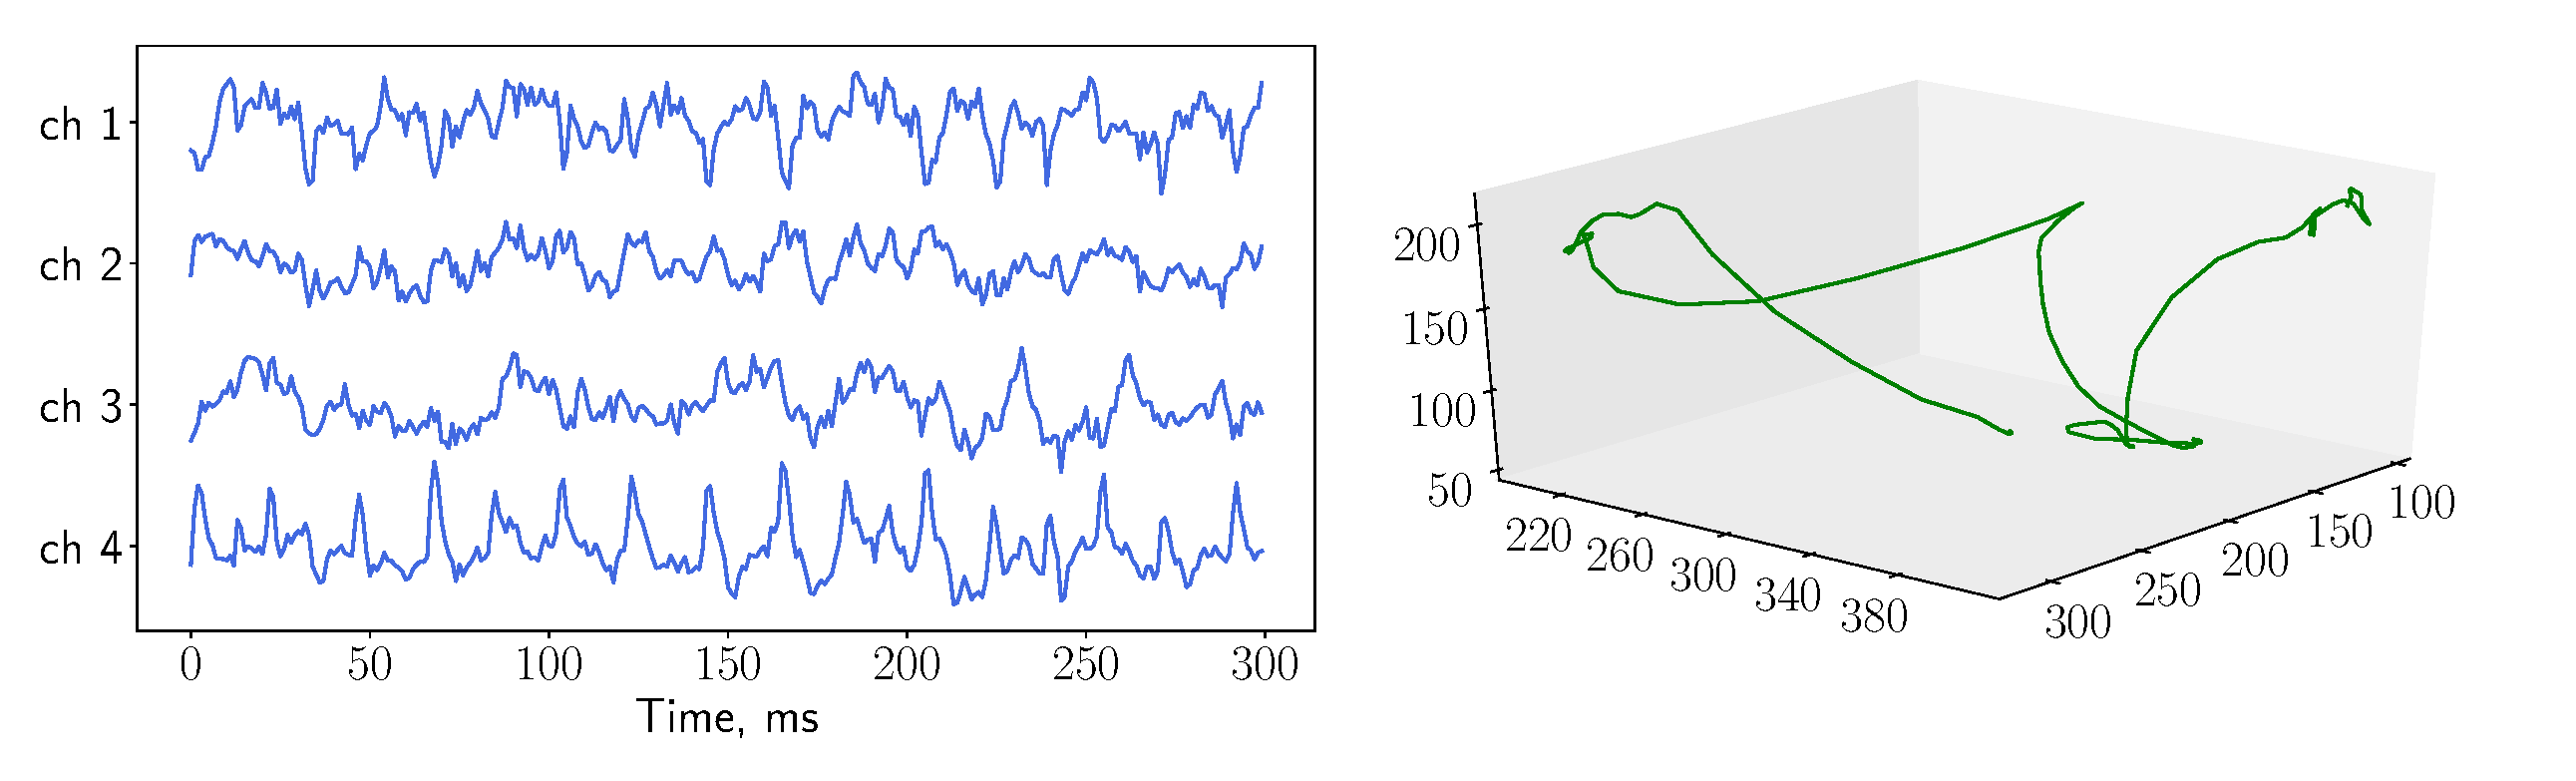
\includegraphics[width=\linewidth]{figs/ch2/ecog_data}
	\caption{Сигналы мозга (левый график) и 3D координаты руки (правый график)}
	\label{ch1:fig:ecog_data}
\end{figure}

Введём среднеквадратичную ошибку для некоторых матриц $\mathbf{A} = [a_{ij}]$ и $\mathbf{B} = [b_{ij}]$
\[
\text{MSE} (\mathbf{A}, \mathbf{B}) = \sum_{i,j} (a_{ij} - b_{ij})^2.
\]
Для оценивания качества аппроксимации вычисляется значение нормированной среднеквадратичной ошибки
\begin{equation}
\text{NMSE}(\bY,  \mathbf{\hat{Y}}) = \frac{\text{MSE} (\bY, \mathbf{\hat{Y}})}{\text{MSE} (\bY, \mathbf{\bar{Y}})},
\label{ch1:eq:nmse}
\end{equation}
где $\mathbf{\hat{Y}}$~--- прогноз модели, $\mathbf{\bar{Y}}$~--- константный прогноз средним значением по столбцам матрицы.

\subsection*{Данные потребления электроэнергии}

Для нахождения оптимальной размерности $l$ латентного пространства все данные потребления электроэнергии были разбиты на обучающую и валидационную части. 
Обучающая выборка состоит из $700$ объектов, валидационная из $370$. Зависимость нормированной квадратичной ошибки~\eqref{ch1:eq:nmse} от размерности $l$ латентного пространства представлена на Рис.~\ref{ch1:fig:energy_n_comp}. 
Сначала ошибка резко падает при увеличении размерности скрытого пространства, а затем стабилизируется.

\begin{figure}[ht]
	\centering
	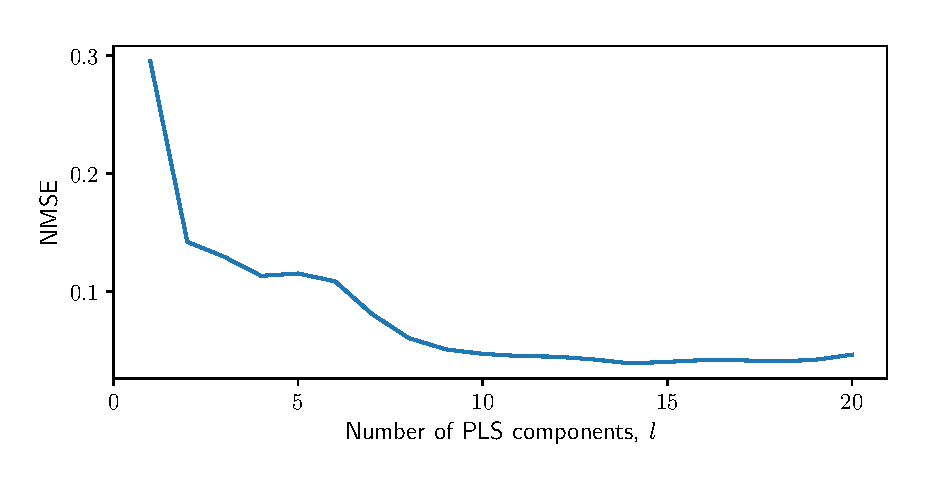
\includegraphics[width=0.75\linewidth]{figs/ch1/energy_n_comp}
	\caption{Прогноз потребления электроэнергии алгоритмом PLS при размерности латентного пространства $l$=14}
	\label{ch1:fig:energy_n_comp}
\end{figure}

Минимальная ошибка наблюдается при $l=14$. 
Построим прогноз потребления электроэнергии при данном $l$. 
Результат аппроксимации изображен на Рис.~\ref{ch1:fig:energy_prediction}. Алгоритм PLS восстановил авторегрессионную зависимость и обнаружил дневную сезонность.

\begin{figure}[ht]
	\centering
	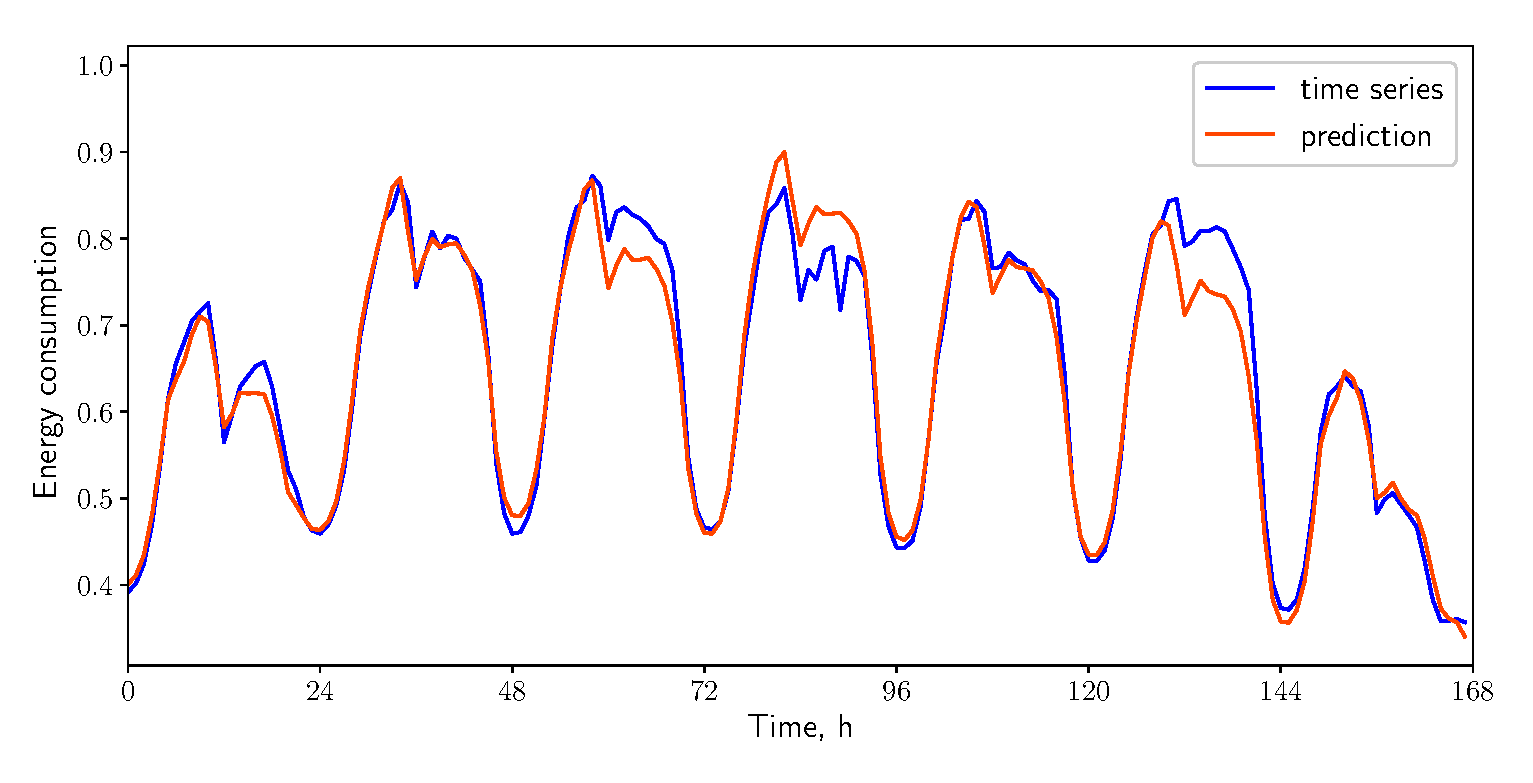
\includegraphics[width=0.95\textwidth]{figs/ch1/energy_prediction}
	\caption{Зависимость ошибки от размерности латентного пространства для данных потребления электроэнергии}
	\label{ch1:fig:energy_prediction}
\end{figure}

\subsection*{Данные электрокортикограммы}

На Рис.~\ref{ch1:fig:ecog_n_comp} представлена зависимость нормированной квадратичной ошибки~\eqref{ch1:eq:nmse} от размерности латентного пространства. Ошибка аппроксимации меняется незначительно при $l > 5$.
Таким образом совместное описание пространственно-временного спектрального представления объектов и пространственного положения руки может быть представлено вектором размерности $l \ll n$.
Зафиксируем $l = 5$. 
Пример аппроксимации положения руки изображен на Рис.~\ref{ch1:fig:ecog_prediction}. 
Сплошными линиями изображены истинные координаты руки по всем осям, пунктирными линиями показана аппроксимация методом PLS.
 
\begin{figure}[ht]
	\centering
	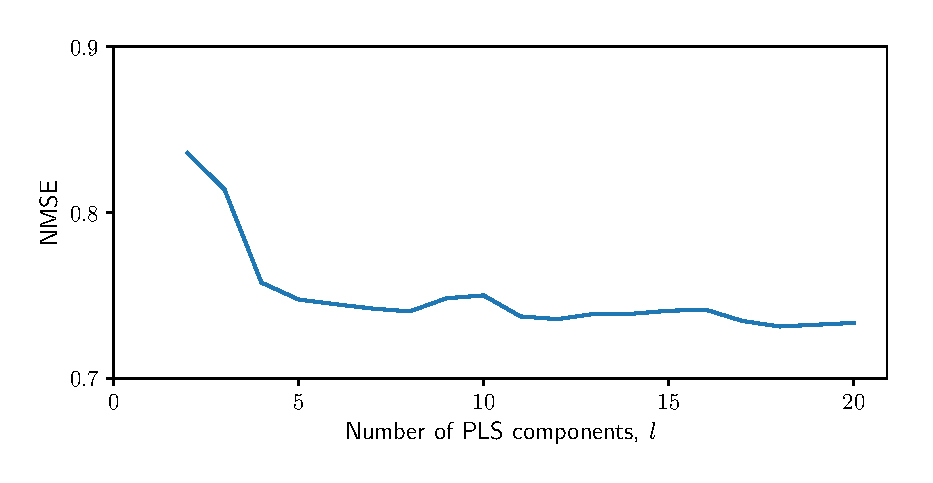
\includegraphics[width=0.75\linewidth]{figs/ch1/ecog_n_comp}	
	\caption{Зависимость ошибки от размерности латентного пространства для данных ECoG}
	\label{ch1:fig:ecog_n_comp}
\end{figure}

\begin{figure}[ht]
	\centering
	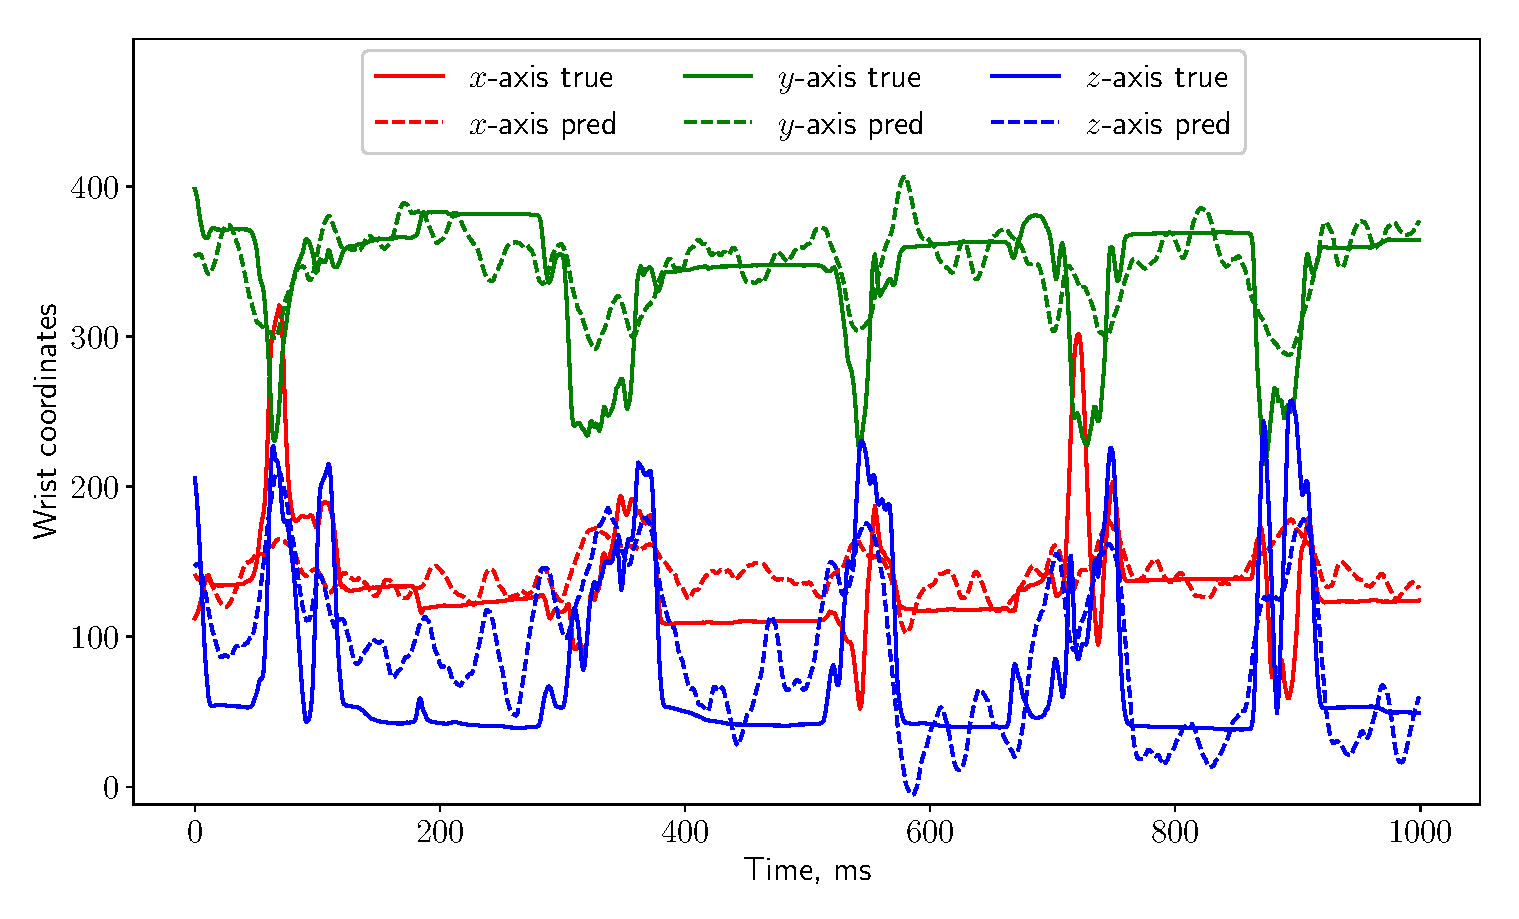
\includegraphics[width=\textwidth]{figs/ch1/ecog_prediction}
	\caption{Прогноз движения руки данных ECoG алгоритмом PLS при размерности латентного пространства $l=5$}
	\label{ch1:fig:ecog_prediction}
\end{figure}

